%\title{LaTeX Portrait Poster Template}
%%%%%%%%%%%%%%%%%%%%%%%%%%%%%%%%%%%%%%%%%
% a0poster Portrait Poster
% LaTeX Template
% Version 1.0 (22/06/13)
%
% The a0poster class was created by:
% Gerlinde Kettl and Matthias Weiser (tex@kettl.de)
% 
% This template has been downloaded from:
% http://www.LaTeXTemplates.com
%
% License:
% CC BY-NC-SA 3.0 (http://creativecommons.org/licenses/by-nc-sa/3.0/)
%
%%%%%%%%%%%%%%%%%%%%%%%%%%%%%%%%%%%%%%%%%

%----------------------------------------------------------------------------------------
%	PACKAGES AND OTHER DOCUMENT CONFIGURATIONS
%----------------------------------------------------------------------------------------

\documentclass[a0,portrait]{a0poster}

\usepackage{multicol} % This is so we can have multiple columns of text side-by-side
\usepackage{multirow}
\columnsep=100pt % This is the amount of white space between the columns in the poster
\columnseprule=3pt % This is the thickness of the black line between the columns in the poster

\usepackage[svgnames]{xcolor} % Specify colors by their 'svgnames', for a full list of all colors available see here: http://www.latextemplates.com/svgnames-colors

\usepackage{times} % Use the times font
%\usepackage{palatino} % Uncomment to use the Palatino font

\usepackage{graphicx} % Required for including images
\graphicspath{{figures/}} % Location of the graphics files
\usepackage{booktabs} % Top and bottom rules for table
\usepackage[font=small,labelfont=bf]{caption} % Required for specifying captions to tables and figures
\usepackage{amsfonts, amsmath, amsthm, amssymb} % For math fonts, symbols and environments
\usepackage{wrapfig} % Allows wrapping text around tables and figures

\usepackage{titlesec}
\titleformat{\section}[block]{\Large\bfseries\filcenter}{}{1em}{}
\titleformat{\subsection}[hang]{\bfseries\large\filcenter}{}{1em}{}

\newcommand{\tr}{\operatorname{Tr}}
\newcommand{\re}{\operatorname{Re}}
\newcommand{\im}{\operatorname{Im}}
\newcommand{\C}{\mathbb{C}}
\newcommand{\R}{\mathbb{R}}
\newcommand{\ID}{\mathbb{I}}
\newcommand{\rf}{\mathcal{R}_5^{\mathbf{sp}}}
\newcommand{\hQpm}{\hat Q^{\pm}}
\newcommand{\hWpm}{\hat W^{\pm}}
\newcommand{\hQp}{\hat Q^{+}}
\newcommand{\hQm}{\hat Q^{-}}
\newcommand{\hWp}{\hat W^{+}}
\newcommand{\hWm}{\hat W^{-}}
\newcommand{\Wpm}{W^{\pm}}
\newcommand{\Qpm}{Q^{\pm}}
\newcommand{\Qp}{Q^{+}}
\newcommand{\Qm}{Q^{-}}
\newcommand{\Wp}{W^{+}}
\newcommand{\Wm}{W^{-}}
\newcommand{\Qnd}{Q_{\textrm{ND}}}
\newcommand{\Tee}{T_{ee}}
\newcommand{\Too}{T_{oo}}
\newcommand{\Moe}{M_{oe}}
\newcommand{\Moo}{M_{oo}}
\newcommand{\Meo}{M_{eo}}
\newcommand{\Mee}{M_{ee}}
\newcommand{\order}{\mathcal{O}}

\newcommand{\Sg}{S_\mathrm{G}}
\newcommand{\Sdeg}{S_\mathrm{deg}}
\newcommand{\Smusig}{S_{\mu_\sigma}}
\newcommand{\Sdel}{S_\delta}
\newcommand{\mudel}{\mu_\delta}
\newcommand{\musig}{\mu_\sigma}
\newcommand{\mutilsig}{\tilde{\mu}_\sigma}
\newcommand{\mutildel}{\tilde{\mu}_\delta}
\newcommand{\mul}{\mu_\ell}
\newcommand{\D}{\mathcal{D}}
\newcommand{\dtau}{\delta\tau}

\newcommand{\csw}{c_\mathrm{sw}}
\newcommand{\mpcac}{m_\mathrm{PCAC}}
\newcommand{\Ntraj}{N_\mathrm{traj}}
\newcommand{\Nmeas}{N_\mathrm{meas}}
\newcommand{\Nconf}{N_\mathrm{conf}}
\newcommand{\Mpi}{M_{\pi^\pm}}
\newcommand{\Mphyspi}{M_{\pi^\pm}^\mathrm{phys}}
\newcommand{\Fpi}{f_{\pi^\pm}}
\newcommand{\Mpin}{M_{\pi^0}}
\newcommand{\Mpinc}{M_{\pi^{(0,c)}}}
\newcommand{\ld}{\mathrm{(LD)}}
\newcommand{\cd}{\mathrm{(CD)}}

\newcommand{\fnabla}{\nabla^\mathrm{f}}
\newcommand{\bnabla}{\nabla^\mathrm{b}}

\newcommand{\mps}{M_\mathrm{P}}
\newcommand{\ps}{\mathrm{P}}
\newcommand{\mpi}{M_\pi}
\newcommand{\mphyspi}{M_{\pi}^\mathrm{phys}}
\newcommand{\fps}{f_\mathrm{P}}
\newcommand{\fpi}{f_\pi}
\newcommand{\mcrit}{m_\mathrm{crit}}
\newcommand{\mw}{m_\mathrm{W}}
\newcommand{\kc}{\kappa_c}
\newcommand{\mn}{M_\mathrm{N}}
\newcommand{\dof}{\mathrm{dof}}

\newcommand{\lmin}{\lambda_\mathrm{min}}
\newcommand{\lmax}{\lambda_\mathrm{max}}
\newcommand{\qcdlambda}{\Lambda_\mathrm{QCD}}

\newcommand{\chipt}{$\chi$PT}
\newcommand{\wchipt}{W$\chi$PT}
\newcommand{\wtmchipt}{Wtm$\chi$PT}

\newcommand{\dingcircle}{\ding{108}}
\newcommand{\dingsquare}{\ding{110}}
\newcommand{\dingrhombus}{\ding{117}}
\newcommand{\dingtriangle}{\ding{115}}

\newcommand{\mev}{~\mathrm{MeV}}
\newcommand{\gev}{~\mathrm{GeV}}
\newcommand{\fm}{~\mathrm{fm}}

\newcommand{\nmev}{\mathrm{MeV}}
\newcommand{\ngev}{\mathrm{GeV}}
\newcommand{\nfm}{\mathrm{fm}}

\newcommand{\Fav}{\|F\|_\mathrm{av}^2}
\newcommand{\Fmax}{\|F\|_\mathrm{max}^2}
\newcommand{\Fsq}{\|F\|^2}
\newcommand{\mutil}{\tilde{\mu}}
\newcommand{\rhotil}{\tilde{\rho}}
\newcommand{\ctil}{\tilde{c}_\mathrm{sw}}

\newcommand{\talkcite}[1]{{\footnotesize \textcolor{blue}{[#1]}}}

\newcommand{\backupbegin}{
   \newcounter{finalframe}
   \setcounter{finalframe}{\value{framenumber}}
}
\newcommand{\backupend}{
   \setcounter{framenumber}{\value{finalframe}}
}

% full page width float
%   \checkoddpage
%   \edef\side{\ifoddpage l\else r\fi}%
%   \makebox[\textwidth][\side]{%
%   \begin{minipage}{1.35\linewidth}
%   \end{minipage}
%   }%

% margin figure
% \marginpar{
%   \centering
%   \includegraphics[width=\linewidth]{}
%   \captionof{figure}[]{}
%   \label{}
% }

% \newtcolorbox{hpcablock}[2][]{%
%   left=3pt,
%   right=3pt,
%   top=3pt,
%   bottom=3pt,
%   colback=bg,
%   colframe=structure!100,
%   fonttitle=\sffamily,
%   coltitle=structure!100,
%   colbacktitle=structure!10,
%   enhanced,
%   attach boxed title to top,
%   title=#2,
%   #1}

% \newtcolorbox{hpcaexampleblock}[2][]{%
%   left=3pt,
%   right=3pt,
%   top=3pt,
%   bottom=3pt,
%   colback=bg,
%   colframe=example text.fg!100,
%   fonttitle=\sffamily,
%   coltitle=example text.fg!100,
%   colbacktitle=example text.fg!10,
%   enhanced,
%   attach boxed title to top left,
%   title=#2,
%   #1}

% \newtcolorbox{hpcaalertblock}[2][]{%
%   left=3pt,
%   right=3pt,
%   top=3pt,
%   bottom=3pt,
%   colback=bg,
%   colframe=alert!100,
%   fonttitle=\sffamily,
%   coltitle=alert!100,
%   colbacktitle=alert!10,
%   enhanced,
%   attach boxed title to top left,
%   title=#2,
%   #1}


\begin{document}

%----------------------------------------------------------------------------------------
%	POSTER HEADER 
%----------------------------------------------------------------------------------------

% The header is divided into two boxes:
% The first is 75% wide and houses the title, subtitle, names, university/organization and contact information
% The second is 25% wide and houses a logo for your university/organization or a photo of you
% The widths of these boxes can be easily edited to accommodate your content as you see fit

% full affiliation list
% \newcommand{\Bern}{Institute for Theoretical Physics, Albert Einstein Center for Fundamental Physics,\\University of Bern, Sidlerstrasse 5, CH-3012 Bern, Switzerland}
% \newcommand{\hiskp}{HISKP (Theory), Rheinische Friedrich-Wilhelms-Universit\"at Bonn,\\Nussallee 14-16, 53115 Bonn, Germany}
% \newcommand{\hpca}{High Performance Computing and Analytics Lab, Rheinische Friedrich-Wilhelms-Universit\"at Bonn,\\ Friedrich-Hirzebruch-Allee 8, 53115 Bonn, Germany}
% \newcommand{\CyprusU}{Department of Physics, University of Cyprus, 20537 Nicosia, Cyprus}
% \newcommand{\CyprusI}{Computation-based Science and Technology Research Center, The Cyprus Institute,\\20 Konstantinou Kavafi Street, 2121 Nicosia, Cyprus}
% \newcommand{\Jena}{University of Jena, Institute for Theoretical Physics, Max-Wien-Platz 1, D-07743 Jena, Germany}
% \newcommand{\Parma}{Dipartimento  di  Scienze  Matematiche,  Fisiche  e  Informatiche,  Universit\`a  di  Parma  and  INFN, Gruppo  Collegato  di  Parma,  Parco  Area  delle  Scienze  7/a  (Campus),  43124  Parma,  Italy}
% \newcommand{\Romadue}{Dipartimento di Fisica and INFN, Universit\`a di Roma ``Tor Vergata",\\Via della Ricerca Scientifica 1, I-00133 Roma, Italy}
% \newcommand{\Romatre}{Dipartimento di Matematica e Fisica, Universit\`a Roma Tre and INFN, Sezione di Roma Tre,\\Via della Vasca Navale 84, I-00146 Rome, Italy}
% \newcommand{\RomatreINFN}{Istituto Nazionale di Fisica Nucleare, Sezione di Roma Tre,\\Via della Vasca Navale 84, I-00146 Rome, Italy}
% \newcommand{\NIC}{NIC, DESY, Platanenallee 6, D-15738 Zeuthen, Germany}
% \newcommand{\Berlin}{Institut f\"ur Physik, Humboldt-Universit\"at zu Berlin, Newtonstrasse 15, 12489 Berlin, Germany}
    
{\VeryHuge \color{NavyBlue} \textbf{Status of the ETMC ensemble generation effort} \color{Black}\\[1.4cm]} % Title

\begin{minipage}[b]{0.74\linewidth}
    % \Huge\textit{Subtitle}\\[2.4cm] % Subtitle
    \Large \textbf{C.~Alexandrou$^{(a)(b)}$, S.~Bacchio$^{(b)}$, J.~Finkenrath$^{(c)}$, R.~Frezzotti$^{(d)}$ M.~Garofalo$^{(e)}$, B.~Kostrzewa$^{(f)}$, G.~Koutsou$^{(b)}$, S.~Romiti$^{(g)}$, A.~Sen$^{(e)}$, C.~Urbach$^{(e)}$, U.~Wenger$^{(g)}$}\\[0.5cm] % Author(s)
    \large $^{(a)}$ Department of Physics, University of Cyprus, 20537 Nicosia, Cyprus\\
    \large $^{(b)}$ Computation-based Science and Technology Research Center, The Cyprus Institute, 2121 Nicosia, Cyprus\\
    \large $^{(c)}$ Theoretical Physics Department, CERN 1211 Geneva 23, Switzerland\\
    \large $^{(d)}$ Dipartimento di Fisica and INFN, Universit\`a di Roma ``Tor Vergata", I-00133 Roma, Italy\\
    \large $^{(e)}$ Helmholtz-Institut f{\"u}r Strahlen- und Kernphysik (Theorie), University of Bonn, 53115 Bonn, Germany\\
    \large $^{(f)}$ High Performance Computing and Analytics Lab, University of Bonn, 53115 Bonn, Germany\\
    \large $^{(g)}$ Institute for Theoretical Physics, Albert Einstein Center for Fundamental Physics, University of Bern, CH-3012 Bern, Switzerland\\
\end{minipage}
%
\begin{minipage}[b]{0.26\linewidth}
    % \includegraphics[width=7cm]{logo.png}\ 
    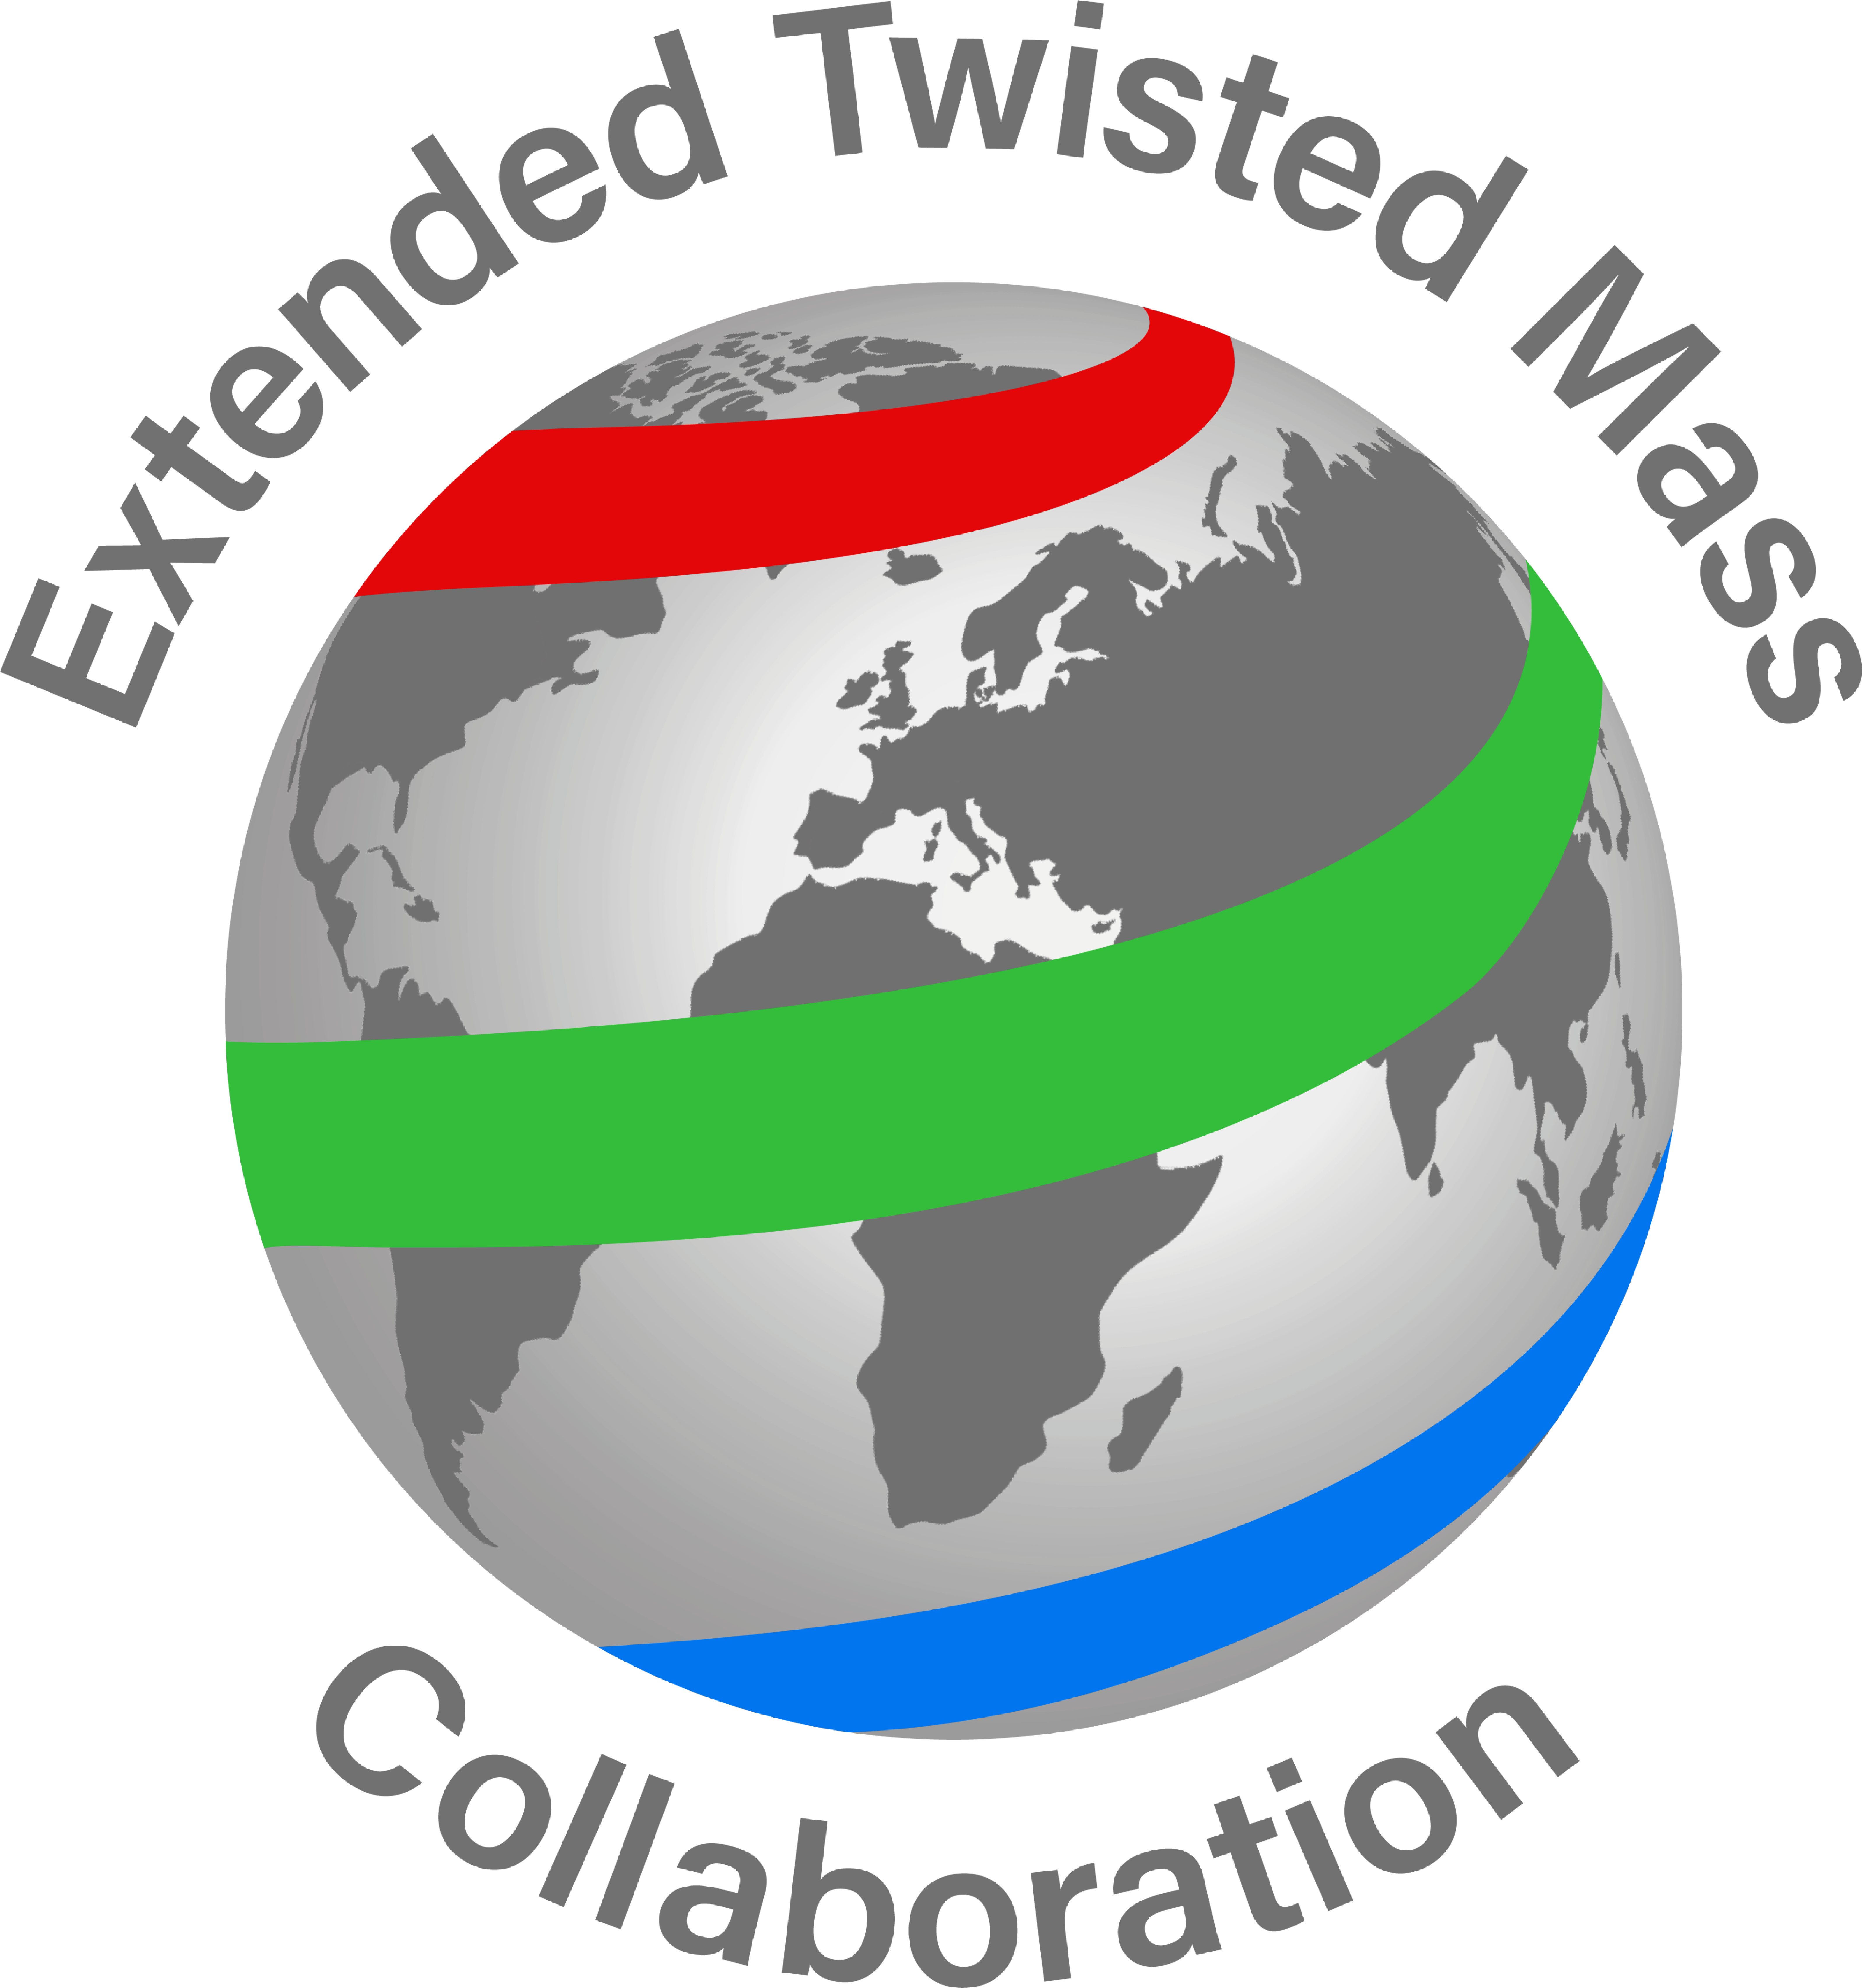
\includegraphics[width=15cm]{figures/Logo_ETMC_RGB.pdf}
\end{minipage}

\vspace{1cm} % A bit of extra whitespace between the header and poster content

%----------------------------------------------------------------------------------------

\begin{multicols}{2} % This is how many columns your poster will be broken into, a portrait poster is generally split into 2 columns

    %----------------------------------------------------------------------------------------
    %	ABSTRACT
    %----------------------------------------------------------------------------------------

    \color{Navy} % Navy color for the abstract

%    \begin{abstract}
%        We report the status of the ensemble generation effort of the Extended Twisted Mass Collaboration towards
%        controlled continuum and infinite volume extrapolations for a variety of physical observables through simulations employing Nf = 2 + 1 + 1 Wilson clover twisted mass fermions at physical quark masses using five
%        lattice spacings. We further give an update on the status of the tmLQCD software suite. Through extensions
%        of the QUDA lattice QCD library and a corresponding interface in tmLQCD, we are able to offload a significant portion of our HMC to GPUs, enabling efficient simulations on the current generation of heterogeneous
%        machines.
%    \end{abstract}
    %----------------------------------------------------------------------------------------
    %	INTRODUCTION
    %----------------------------------------------------------------------------------------

    \color{Black} % SaddleBrown color for the introduction
    \subsection*{Introduction}
    The $Nf =2+1+1$ path integral for twisted mass Wilson clover (tmWc) fermions \cite{Frezzotti:2003ni,Frezzotti:2004wz,Sheikholeslami:1985ij} is
    \begin{flalign*}
      Z= \int \mathcal{D}U \mathcal{D}\chi \mathcal{D}\bar\chi \,e^{-S_\mathrm{gauge}-\bar \chi D_\ell\chi - \bar \chi D_h \chi } \,, &  &
    \end{flalign*}
    where $D_\ell$ is the Dirac operator for a doublet of light mass-degenerate quarks and $D_h$ is the Dirac operator for a non-degenerate doublet corresponding to the strange and charm contributon:
    \begin{flalign*}
        \label{eq:eosw0}
        D_\ell = (\Dsw[U] + m_0)\ 1_f + i \mu_\ell\gamma_5\tau^3\, ,\quad\quad
        D_h = (\Dsw[U] + m_0)\ 1_f + i\bar\mu\gamma_5\tau^3 - \bar\epsilon \tau^1 &  &
    \end{flalign*}
    where $\Dsw$ is the Wilson clover operator while $m_0$, $\mu_\ell$, $\mubar$ and $\epsbar$ are the various untwisted and twisted mass parameters.
    We employ Hasenbusch mass-preconditioning \cite{Hasenbusch:2001ne} to split the light quark determinant and and rational HMC \cite{Clark:2006fx} for the non-degenerate. Even-odd preconditioning is used throughout.

    % The various inversions are performed using the most appropriate solver for each monomial.
    % \vspace{1cm}
    % \begin{tabular}{p{0.3\linewidth}p{0.7\linewidth}}
    %   \centering $\frac{1}{\What_{+}(\rho_t) \What_{-}(\rho_t)}$ & double-half mixed-precision CG \\
    %   \centering $\What_{-}(\rho_t) \frac{1}{\What_{+}(\rho_b) \What_{-}(\rho_b)} \What_{+}(\rho_t)$ & double-half mixed precision CG or multigrid-preconditoned GCR depending on $\rho_b$ \\
    %   \centering $\prod_{i=n_\ell}^{n_k} \frac{ \Qhat^2_h + a_{2i-1} }{ \Qhat^2_h + a_{2i} }$ & single precision multi-shift CG with double-half precision shift-by-shift refinement 
    % \end{tabular}
    % Integrating fermion variables and using Even/odd Preconditioning
    % \begin{flalign*}
    %     Z= \int DU  \,e^{-S_{gauge} }\det{\left(M_{ee}^+M_{ee}^-\right)}
    %     \det{(\hat Q_{+}\hat Q_{-})}
    %     \det{(\hat Q_h)} \det{(M_{ee}^{h})} &  &
    % \end{flalign*}
    % with the degenerate operator written in terms of the even/odd part of the operator
    % \begin{flalign*}
    %     \hQpm = \gamma_5 \left[  \Moo   - \Moe \Mee^{-1} \Meo \right] \,,\quad \quad
    %     \Mee =1 + 2\kappa c_{SW} T_{ee} + i\tilde\mu\gamma_5 \,, \quad \quad M_{deg} =\gamma_5 \begin{pmatrix}
    %                                                                                                M_{ee} & M_{eo} \\
    %                                                                                                M_{oe} & M_{oo} \\
    %                                                                                            \end{pmatrix} &  &
    % \end{flalign*}
    % while the non-degenerate operator is a two-flavour operators
    % \begin{flalign*}
    %     \hat	Q_h = \gamma_5 \left[ ( \Moo^h + i \mu_\sigma \gamma_5 \tau^3 - \mu_\delta \tau^1 ) - \Moe^h (\Mee^h + i \mu_\sigma \gamma_5 \tau^3 - \mu_\delta \tau^1 )^{-1} \Meo^h \right] &  &
    % \end{flalign*}

    % Applaying Hasenbusch trick \cite{Hasenbusch:2001ne} for the degenerate and Rational HMC \cite{Clark:2006fx} for the non degenerate operator
    % we get
    % \begin{multline*}
    %     Z= \int DU  \,e^{-S_{gauge} }\det{\left(M_{ee}^+M_{ee}^-\right)}
    %     \det{(\hat W_{+}\hat W_{-})}	\det{(\hat W_{+}^{-1}\hat Q_+\hat Q_-\hat W_{-}^{-1})}...\,\\
    %     \det{(M_{ee}^{h})}
    %     {\det{(  r_1(\hat Q_h) )}\det{(  r_2(\hat Q_h) )}...\,\det{(|\hat Q_h|{\cal R}(\hat Q_h)}}
    % \end{multline*}
    % with the operator
    % $\hWpm(\rho) = \hQpm \pm i \rho$ s.t. $\hWp(\rho) \hWm(\rho) = \hQp \hQm +\rho^2$ such that the clover inverse $\rho$-independent.
    % The rational approximation is
    % \begin{equation*}
    %     \mathcal{R}(\hat Q_h^2) = \prod_{i=1}^{N} \frac{\hat Q^2_h + a_{2i-1}}{\hat Q^2_h + a_{2i}}=\prod_{i=1}^{N} r_i(\hat Q_h) \approx \frac{1}{\sqrt{\hat Q_h^2}}
    % \end{equation*}
    % with $N \approx 10$, with $\mathcal{R}$ split across 2-3 monomials $r_i(\hat Q_h)$ on 2-3 timescales (usually 3).
    % Exponentiating the determinants we get the action used in the HMC \cite{Duane:1987de}
    % \begin{flalign*}
    %     Z= \int DU D\phi D\phi^*  \,e^{-S_{gauge} } e^{-S_{det}}
    %     e^{-S_{PF}}  e^{-S_{PF}^1}...\,
    %     {e^{-S_{det}^h}}
    %     {e^{-S_{det}^h}}
    %     e^{-S_{PF}^{1h}} e^{-S_{PF}^{2h}}...\,
    %     e^{-S_{corr}}\,.
    % \end{flalign*}
    % The corresponding equation of motion to be integrated in the HMC are
    % \begin{align*}
    %     \partial_t U   & =\Pi                \\
    %     \partial_t \Pi & =-\delta S_{gauge}-
    %     \delta S_{det} - \delta S_{PF} - \delta S_{PF}^1 -...-
    %     \delta S^h_{det} -\delta S^{1h}_{PF} - \delta S^{2h}_{PF}-...-
    %     \delta S_{corr}\,.
    % \end{align*}


    \subsection*{Overview of current ensembles}
    \begin{center}
      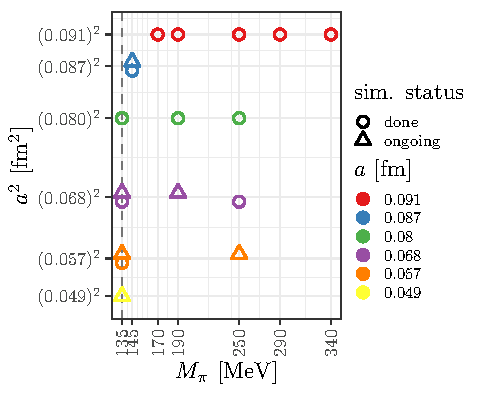
\includegraphics[height=15cm]{ensembles_asquared_mpi}\hspace{1cm}
      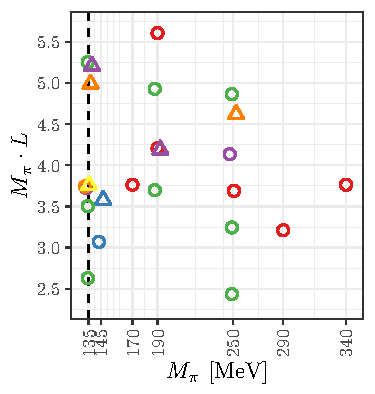
\includegraphics[height=15cm]{ensembles_L_vs_mpi}
    \end{center}
    \begin{itemize}
      \item 7 approximate pion mass values: 135 MeV $\leq M_\pi \leq $ 340 MeV
      \item 6 lattice spacings: 0.049 fm $\leq a \leq$ 0.091 fm
      \item 5 lattice spacings close to or at the physical pion mass
      \item multiple volumes at many pion mass points: 2.5 fm $\leq L \leq$ 7.7 fm
    \end{itemize}
    \subsection*{Ensembles close to the physical point}

    \begin{minipage}{0.42\linewidth}
      \begin{center}
        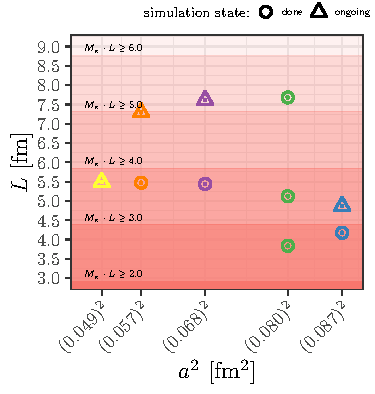
\includegraphics[width=\linewidth]{ensembles_phys_point}
      \end{center}
    \end{minipage}
    \hspace{0.04\linewidth}
    \begin{minipage}{0.52\linewidth}
      \begin{center}
        \textbf{Continuum extrapolaton of $a_\mu^W(s)$ using 3 or 4 lattice spacings}
        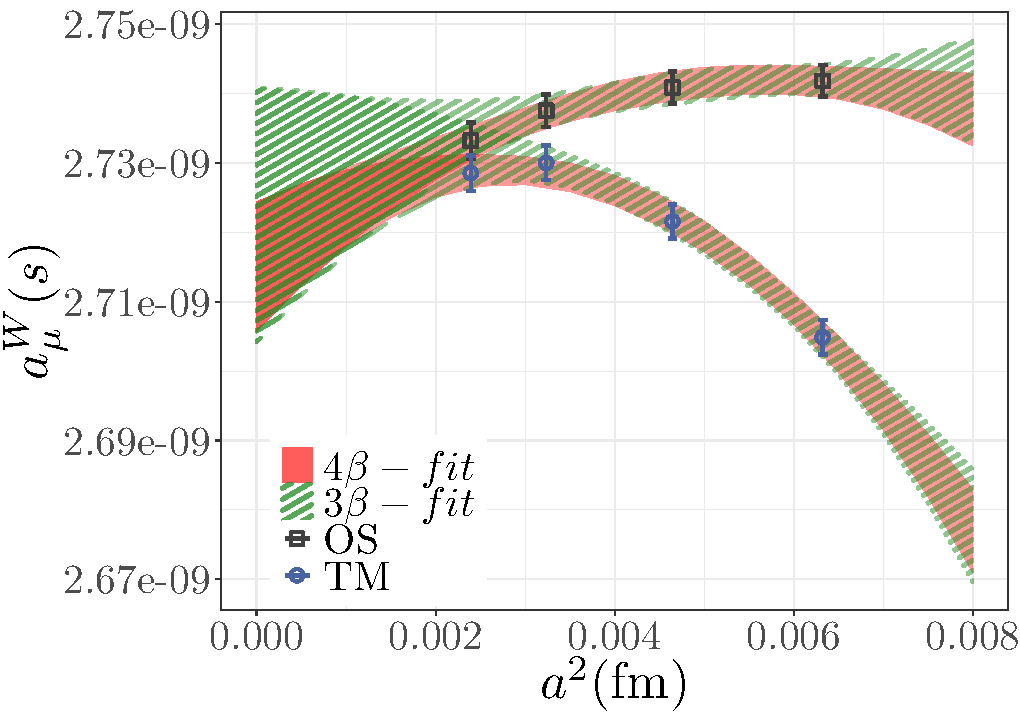
\includegraphics[width=\linewidth]{amu_s_W_a4}
      \end{center}
    \end{minipage}

    \subsection*{Statistical properties close to the physical pion mass}
    \begin{minipage}{0.48\linewidth}
        \centering
        \textbf{\hspace{3cm}Gradient-flowed energy density}\\
        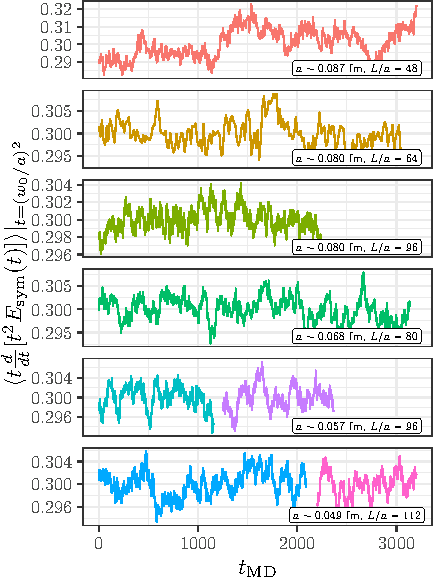
\includegraphics[width=\linewidth,page=1]{data/gf_observables/gf_observables_md_histories}
        \begin{itemize}
            \item Long $\tau_\mathrm{int}$ in $w_0/a$ at coarse lattice spacing, not negligible at fine lattice spacing.
        \end{itemize}
    \end{minipage}
    \hfill
    \begin{minipage}{0.48\linewidth}
        \centering
        \textbf{\hspace{3cm}Topological charge}\\
        \includegraphics[width=\linewidth,page=2]{data/gf_observables/gf_observables_md_histories}
        \begin{itemize}
            \item Topological charge moves well even at $a\approx 0.049 \, \mathrm{fm}$
        \end{itemize}
    \end{minipage}

    \subsection*{Algorithmic choices for the MD Hamiltonian}
    \noindent The molecular dynamics Hamiltonian is decomposed into monomials which are integrated on different time scales according to their contribution to the force using a second-order minimal norm integrator, including a force-gradient term for large volumes, 2MN(FG). The inversions are performed using the most appropriate solver for each monomial.
    \vspace{0.5cm}

    \begin{tabular}{p{0.08\linewidth}p{0.2\linewidth}p{0.3\linewidth}p{0.3\linewidth}}
    \multirow{2}{*}{$\What_\pm(\rho)$} & even-odd & \centering $\frac{1}{\What_{+}(\rho_t) \What_{-}(\rho_t)}$ & double-half mixed precision CG \\
      & mass precon & \centering $\What_{-}(\rho_t) \frac{1}{\What_{+}(\rho_b) \What_{-}(\rho_b)} \What_{+}(\rho_t)$ & multigrid-preconditoned GCR or CG, depending on $\rho$ \\
      $\Qhat_h$ & e/o precon, non-degenerate, RHMC & \centering $\prod_{i=n_\ell}^{n_k} \frac{ \Qhat^2_h + a_{2i-1} }{ \Qhat^2_h + a_{2i} }$ & single precision multi-shift CG with double-half precision shift-by-shift refinement
    \end{tabular}

    %----------------------------------------------------------------------------------------
    %	tmLQCD + QUDA
    %----------------------------------------------------------------------------------------
    \subsection*{tmLQCD + QUDA}

    An efficient usage of GPUs is achieved in tmLQCD via the QUDA library~\cite{Clark:2009wm,Babich:2011np}. As first step in interfacing tmLQCD to QUDA \cite{Kostrzewa:2022hsv} the most expensive part of the HMC, i.e. the inversion of the various Dirac operators and the gauge force were offloaded. In the last year we further offloaded all computations of the fermionic force. In this way, tmLQCD can reach GPU utilizations in excess of 70\% and even up to 90\% depending on the number of available CPU cores per GPU.

    \begin{center}
      \textbf{real-time speedup through increased GPU offloading}\\
      left to right:\\
      CPU only, GPU solves only, GPU $N_f=2$ force, full GPU $N_f=2+1+1$ force
    \end{center}
    \vspace{0.5cm}
    \begin{minipage}{0.5\linewidth}
      \centering
      volume $64^3 \cdot 128$ \@ physical $M_\pi$
      \includegraphics[height=13.5cm,page=2]{data/tmLQCD_performance/quda_speedup}\\
    \end{minipage}
    \begin{minipage}{0.5\linewidth}
      \centering
      volume $112^3 \cdot 224$ \@ physical $M_\pi$
      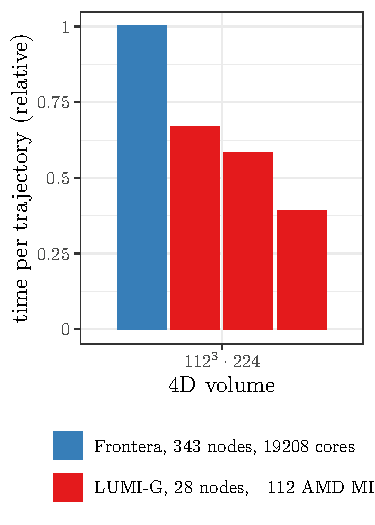
\includegraphics[height=13.5cm,page=1]{data/tmLQCD_performance/quda_speedup}\\
    \end{minipage}

    \begin{minipage}{0.5\linewidth}
      \centering
      Juwels Booster strong scaling $(64^3 \cdot 128)$\\
      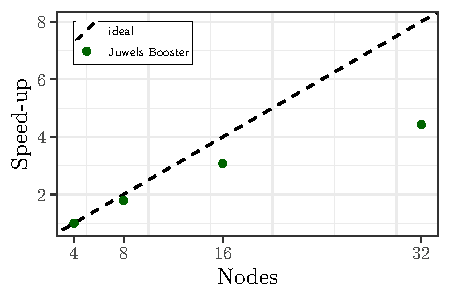
\includegraphics[width=0.80\linewidth,page=1]{data/tmLQCD_scaling/HMC_Scaling}\\
    \end{minipage}
    \begin{minipage}{0.5\linewidth}
      \centering
      LUMI-G strong scaling $(112^3 \cdot 224)$\\
      \includegraphics[width=0.80\linewidth,page=2]{data/tmLQCD_scaling/HMC_Scaling}\\
    \end{minipage}
    
    


    %----------------------------------------------------------------------------------------
    %	CONCLUSIONS
    %----------------------------------------------------------------------------------------

    %\color{SaddleBrown} % SaddleBrown color for the conclusions to make them stand out
    %\section*{Conclusions}
    %\color{Black} % Set the color back to DarkSlateGray for the rest of the content

    %----------------------------------------------------------------------------------------
    %	FORTHCOMING RESEARCH
    %----------------------------------------------------------------------------------------

    \subsection*{Acknowledgments}
    \small 
    We would like to thank the QUDA developers for their tremendous work as well as the many pleasant and productive
    interactions during this and previous efforts. We thank the ETMC for the most enjoyable collaboration. 
    % for part of this work. S.B. and J.F. are supported by the H2020 project PRACE 6-IP (grant agreement No.
    % 82376) and the EuroCC project (grant agreement No. 951740).
    % We acknowledge support by the European Joint Doctorate
    % program STIMULATE grant agreement No. 765048.
    % This work is supported by the Deutsche Forschungsgemeinschaft
    % (DFG, German Research Foundation) and the NSFC through the funds provided to the Sino-German Collaborative
    % Research Center CRC 110 “Symmetries and the Emergence of Structure in QCD” (DFG Project-ID 196253076 - TRR
    % 110, NSFC Grant No. 12070131001).
    We gratefully acknowledge the Gauss Centre for Supercomputing e.V. (www.gauss-centre.eu) for funding this project through computing time on the GCS supercomputer JUWELS Booster at the Jülich Supercomputing Centre.
    We gratefully acknowledge the Swiss National Supercomputing Centre (CSCS) and the EuroHPC Joint Undertaking for awarding this project access to the LUMI supercomputer, owned by the EuroHPC Joint Undertaking, hosted by CSC (Finland) and the LUMI consortium through the Chronos programme under project IDs CH17-CSCS-CYP and CH21-CSCS-UNIBE as well as the EuroHPC Regular Access Mode under project ID EHPC-REG-2021R0095. 
    Some of the simulations were performed on the Luxembourg national supercomputer MeluXina.
    % Some of the runs done for this work were carried out on the Bender GPU cluster
    % at the University of Bonn and we gratefully acknowledge support by the HRZ-HPC team.
    %----------------------------------------------------------------------------------------
    %	REFERENCES
    %----------------------------------------------------------------------------------------

    % \nocite{*} % Print all references regardless of whether they were cited in the poster or not
    \bibliographystyle{plain} % Plain referencing style
    \bibliography{sample} % Use the example bibliography file sample.bib

    %----------------------------------------------------------------------------------------

\end{multicols}
\end{document}
